\LARGE{ \textbf {Лекция №2}}
\Large{ \textbf {Перевод восьмеричной в двоичную и обратно.}}

При переводе используют тот факт что $ 8 = 2^3$, для представления восьмеричной цифры используется 3 разряда.
$6_8 = (110)_2 \quad
8_8 = (100)_2 $
$$ (25,8)_8 = (010101,110)_2 = (10101,11)_2 $$


При обратном преобразовании исходное число разбивают на триады , начиная от двоичной точки ( запятой), при необходимости дописывают незначащие нули.
Затем каждой триаде сопоставляют восьмеричную цифру.
$$ (1010110,0101)_2 = (001)(010)(110),(010)(100) = (126,24)_8     $$

Для перевода шестнадцатиричных чисел в двоичную и обратно используется тот факт, что
$ 16 = 2^4 $.

\Large{ \textbf {Двоичная арифметика.}} \\
Аксиомы двоичной арифметики.\\
Основные операции $ +, -, \cdot .$\\
Сложение\\
$0+0=0\\
0+1=1\\
1+0=1\\
1+1= 10$\\
Вычитание\\
$0-0=0\\
1-0=1\\
1-1=0\\
0-1= 1$ — Происходит заём из старшего разряда.

Умножение\\
$0 \cdot 0=0\\
0 \cdot 1=0\\
1 \cdot 0=0\\
1 \cdot 1=0$\\
\newpage
\Large{ \textbf {Двоичное сложение многоразрядных цифр схоже с правилами сложения десятичных чисел}}\\
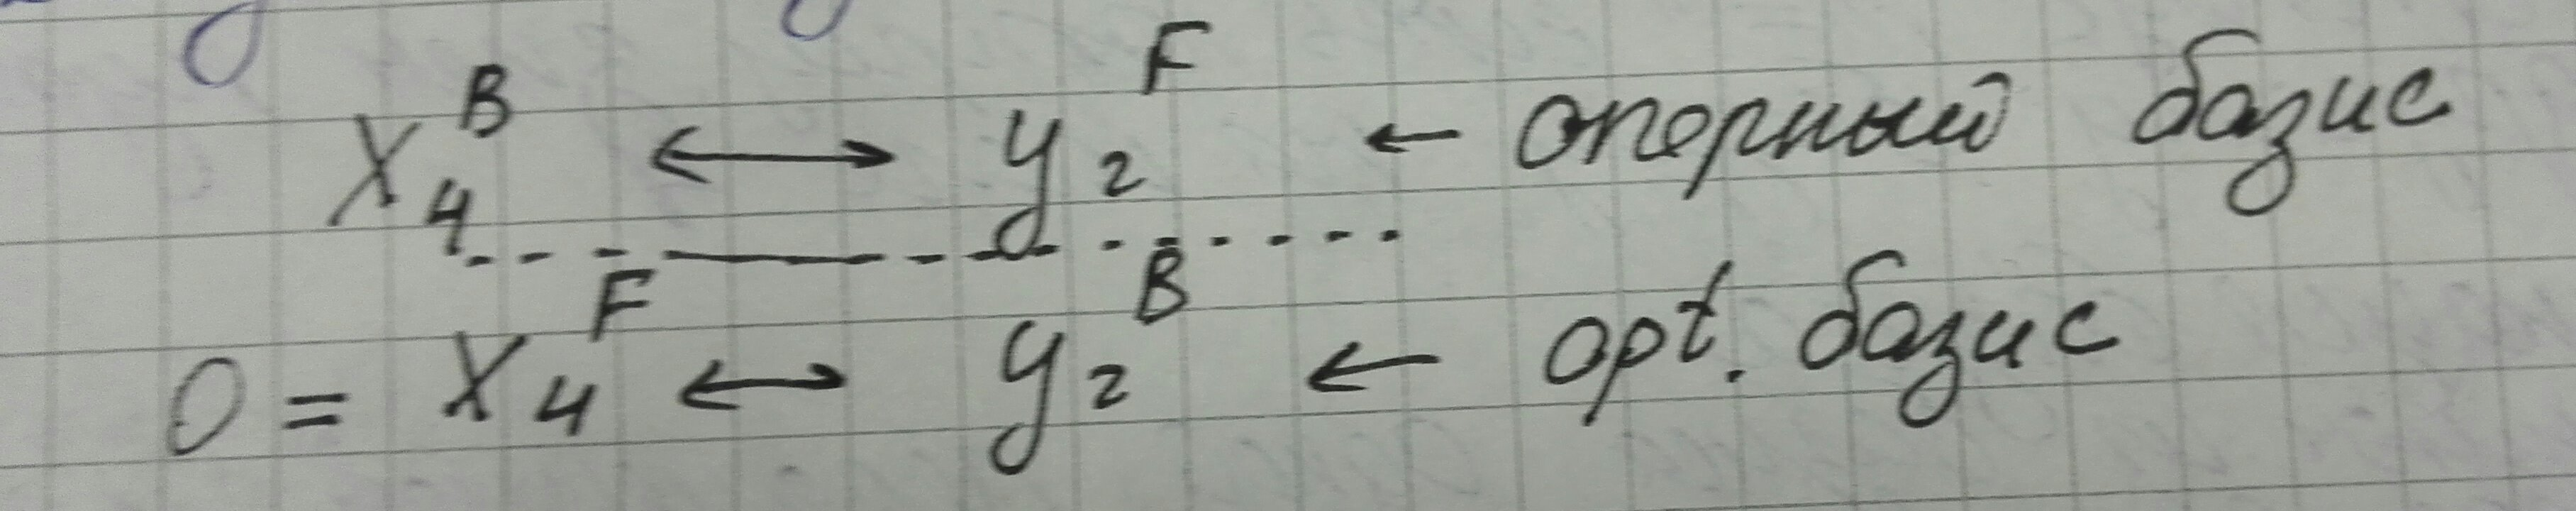
\includegraphics[width=\linewidth]{2}


\Large{ \textbf { Форма представления чисел в ЭВМ}}\\
В ЭВМ принято использовать 2 формы представления чисел.
Представление чисел с фиксированной запятой — естественная форма.
Представление с плавающей запятой — полулогарифмическая форму


Дописать —————————————————----------------------------------------------------—\\
Точка фиксируется либо после младшего разряда, либо перед старшим разрядом.\\
\begin{itemize}
  \item{ Точка фиксируется после младшего разряда.\\
  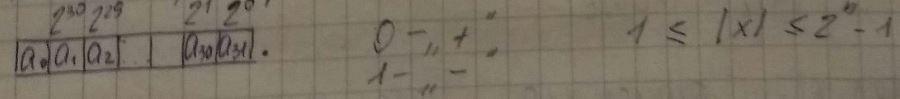
\includegraphics[width=\linewidth]{3}
  $a_0$ — знак числа , 0 — ‘-‘, 1— ‘+’
  }
  \item{Числа по модулю меньшие $ 2_{-n} $ не могут быть отображены и принимаются равными нулю.
Если модуль числа больше 1 , то говорят о переполнении разрядной сетки и овыходе влево.\\
  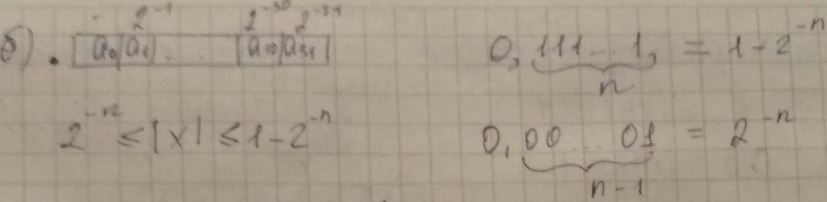
\includegraphics[width=\linewidth]{4}
}
\end{itemize}

\newpage
\Large{ \textbf {Представление чисел с плавающей запятой}}\\
m  — значение мантиссы\\
p -порядок числа\\
b — основание системы счисления\\
$$ m \cdot b^p $$
$$(a \cdot 10^n) \cdot  (b \cdot 10^m) = a \cdot b  \cdot^{n  m}  $$
$$(a \cdot 10^n)  /  (b \cdot 10^m) = \frac{a}{b} \cdot^{n - m}  $$
$$(a \cdot 10^n)  +  (b \cdot 10^m) =(a'\cdot 10^m) + (b\cdot 10^m)= (a' +b) \cdot^{n  m}  $$

Для хранения таких чисел требуется разбить сетку для хранения мантисс и порядка.
Вводится понятие нормализованного числа: $b_{-1} < m < 1 $ \\
Для нормализованного двоичного числа в старшем разряде находится единица.\\
{\itshapeНормализованное число} представляет это число с максимальной точностью.
Если для хранения используется единичная точность, то при выполнении операций используется двойная точность. Стандарты связанные с нормализованным числом: IEEE  754 - 1985 ,2008.\\
В стандарте 2008 года использованы следующие улучшения: \\
Так как число нормализованно, то всегда начинается с 1, следовательно её можно не хранить. Но мы всегда её подразумеваем. (Эта единица как бы между 8 и 9 разрядом.)\\
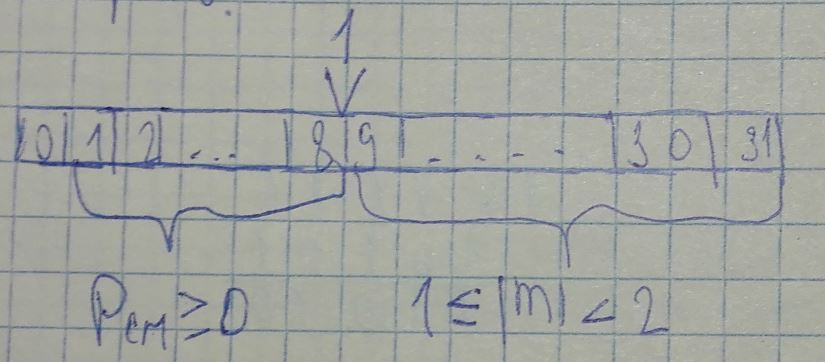
\includegraphics[width=\linewidth]{5} \\
$ P_{CM} \geq  0 \\
P_{CM}  = p + N\\
N = 2^{k-1} - 1 \mbox{в нашем случае k = 8 и N = 127}\\
$
Отметим:
Положительные числа всегда представляют в прямом коде. Прямой код положительного числа совпадает с положительным числом.


\Large{ \textbf {Представление в ЭВМ отрицательных чисел}}
Прямой, обратный и дополнительный коды.

Прямой код отрицательного числа.\\
Все цифровые разряды остаются неизменными, а знаковая часть равна единице.
$
A = - 0,101 \\
A_{pr} =  1,101 \\
$
Для того чтобы сложить числа числа разных знаков нужно много действий:

Алгоритм
\begin{enumerate}
  \item Выяснить какое число по модулю больше
  \item Вычесть из него меньшее
  \item Присвоить результату знак большего по модулю числа
\end{enumerate}
Представление в обратном или дополнительном коде позволяет свести операцию вычитания к операции арифметического сложения кода.

Обратный код получается инвертированием значений цифр в числе.  0 — 1\\
$
A_{obr} =  1,010 \\
A_{obr} = 2 - 2^{-n} - A \\
$
Дополнительный код числа — в разряд заносят единицу в цифровую часть числа заменяют дополнением модуля числа до 2.\\
$
A_{dop} = 2 - A \\
A_{dop} = A_{obr} + 2^{-n} = A_{obr} + \mbox{единица в младший разряд}\\
$
Таким образом дополнительный код получается следующим образом:
|\begin{enumerate}
  \item Добавляем 1 в целую часть
  \item Инвертируем дробную часть
  \item Добавляем 1 в младший разряд
\end{enumerate}
$ A_{dop} = 1,011$
